\section{Durchf\"uhrung}

In   diesem   Versuch   wird    ein    monochromatischer    Laser    durch   ein
Polarisator/Analysator-Paar geschossen und die Lichtintensit\"at wird  gemessen.
Der Polarisator wird ungef\"ahr auf $\SI{0}{\degree}$ gesetzt und bleit so f\"ur
das ganze Experiment.

Zwischen dem Polarisator und Analysator werden  eine $\lambda/2$-Platte und eine
$\lambda/4$-Platte  platziert.  Es   werden   bei   verschiedenen   Winkeln  die
Durchlasskennlinien  gemessen,   indem  der  Analysator  gedreht  wird  und  die
austretende Intensit\"at gemessen wird.

Als       monochromatische        Quelle        wird       ein       He-Ne-Laser
($\lambda=\SI{632.8}{\nano\meter}$) verwendet. In der Letzten Aufgabe  wird  ein
Gr\"uner  Laserpointer verwendet (diodengepumpter, frequenzverdoppler, NdYAG mit
$\lambda=\SI{532}{\nano\meter}$).

Die Polarisatoren  sind  Glan-Thompson  Prismen  in  Pr\"azisionsdrehaltern. Die
L\"oschungsverh\"altnis (extinction ratio) ist in gekreuzter Stellung besser als
$10^{-5}$.

\begin{figure}[H]
    \centering
    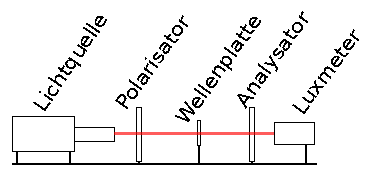
\includegraphics[width=.7\linewidth]{images/messaufbau.pdf}
    \caption{Messaufbau}
    \label{fig:messaufbau}
\end{figure}


\subsection{Berechnung einer Viertelwellenplatte}

Die Dicke einer $\lambda/4$-Wellenplatte erster  Ordnung  ($m=0$) muss berechnet
werden. Die Brechungsindizes von  Quartz  sind  $n_e=1.55328$ und $n_0=1.54418$.

Die Dicke l\"asst sich einfach mit folgender Formel berechnen.

\begin{equation}
    d = \frac{\lambda_0}{4\left(n_e-n_0\right)} = \SI{15.663}{\micro\meter}
\end{equation}

Wobei  $\lambda_0$  die  Wellenl\"ange  des  Lichts  im  Vakuum  ist.  Es  wurde
$\lambda_0=\SI{632.8}{\nano\meter}$ gew\"ahlt.

Dieses    Resultat    scheint    sich    mit    einem    Online-Calculator    zu
decken.\cite{ref:waveplate_calculator}.


\subsection{Durchlasskennlinie Polarisator/Analysator-Paar}

Die  Durchlasskennlinie  des  Polarisator/Analysator-Paars  wurde  experimentell
gemessen. Dabei wurde  die  Messeinrichtung  in  Abbildung  \ref{fig:messaufbau}
verwenden, aber ohne Wellenplatte.

Die  Lichtintensit\"at   wurde   f\"ur   verschiedene   Winkeleinstellungen  des
Analysators gemessen.


\subsection{Ausl\"oschwinkel Halbwellenplatte}

In  dieser   Aufgabe   wurde   wie   in   Abbildung   \ref{fig:messaufbau}  eine
Halwellenplatte    zwischen   Polarisator   und   Analysator   eingebaut.    Die
Halbwellenplatte wurde zwischen $\SI{0}{\degree}$ und $\SI{90}{\degree}$ gedreht
und der Ausl\"oschwinkel des  Analysators  wurde  f\"ur  jede  Winkeleinstellung
bestummen.

Gem\"ass  Theorie  m\"usste die Polarisationsebene um den doppelten  Winkel  der
Halbwellenplatte drehen.


\subsection{Durchlasskennlinien Viertelwellenplatte}

In   dieser   Aufgabe  wurde  wie   in   Abbildung   \ref{fig:messaufbau}   eine
Viertelwellenplatte zwischen Polarisator  und Analysator eingebaut. Es gilt, die
Intensit\"at    $I(\varphi,\vartheta)$     einerseits     in     Funktion    der
Wellenplattenwinkel  $\varphi$,  anderseits in  Funktion  des  Analysatorwinkels
$\vartheta$ zu bestimmen.

Es   wurden  die   Einstellungen   $\varphi=\SI{0}{\degree},   \SI{15}{\degree},
\SI{30}{\degree},      \SI{45}{\degree},      \SI{60}{\degree}$       verwendet.


\subsection{Durchlasskennlinie Viertelwellenplatte bei Gr\"unem Licht}

In   dieser  Aufgabe  wird  auch  wie  in  Abbildung  \ref{fig:messaufbau}  eine
Viertelwellenplatte zwischen  Polarisator  und  Analysator  platziert. Der Laser
wird jedoch mit einer Gr\"unen Laserdiode ersetzt.
Das  heisst dass die $\lambda/4$-Platte gar keine $\lambda/4$-Platte  mehr  ist,
weil sie nicht f\"ur diese Wellenl\"ange  dimensioniert wurde. Als resultat wird
es  nicht  mehr  m\"oglich  sein, ein perfekte Kreispolarisation  zu  erreichen.

Es wird gemessen, wie ``elliptisch'' die Durchlasskennlinie ist.
